\begin{center}
    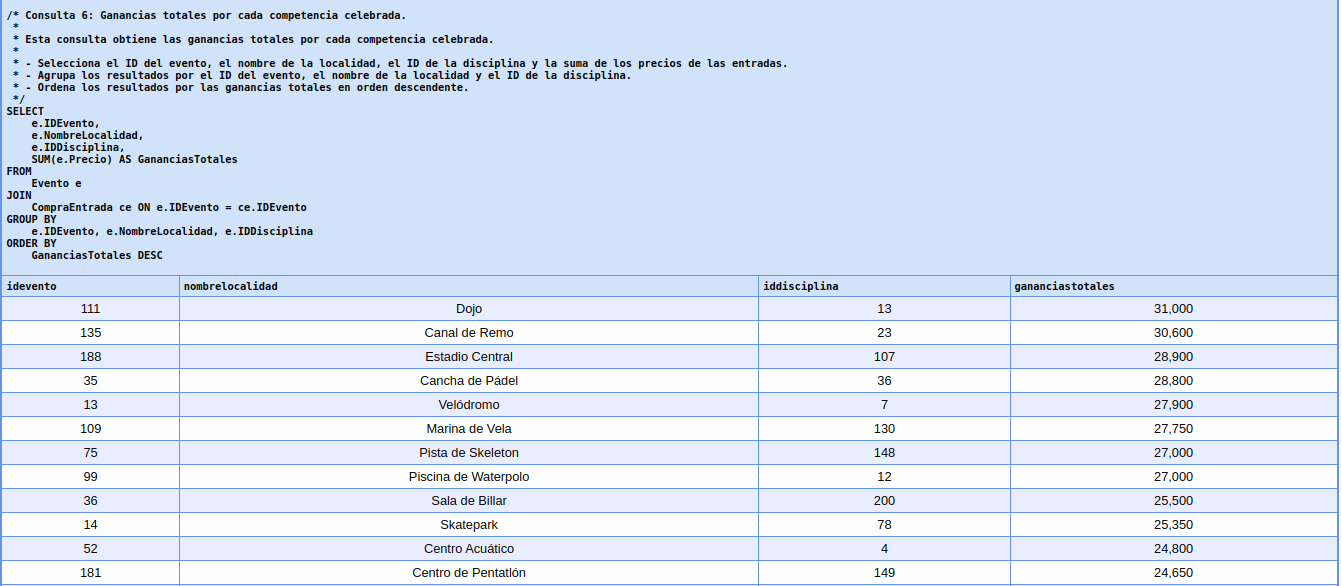
\includegraphics[width=16.5cm]{../resources/Chapters/Consultas/Imagenes/Consulta6.png} 
    
   Consulta 6. Ganancias totales por cada competencia celebrada.
\end{center}

\textbf{Propósito de la consulta}

La consulta tiene como objetivo calcular las ganancias totales generadas por la venta de entradas para cada competencia celebrada. Esto permite identificar qué eventos fueron más rentables y en qué localidades o disciplinas se generaron mayores ingresos.

\textbf{Desglose de la consulta}

\begin{itemize}
   \item \textbf{Selección de columnas (\texttt{SELECT}):}
   \begin{itemize}
       \item \texttt{e.IDEvento}: Identificador único del evento, que permite distinguir cada competencia.
       \item \texttt{e.NombreLocalidad}: Nombre de la localidad donde se celebró el evento.
       \item \texttt{e.IDDisciplina}: Identificador de la disciplina deportiva asociada al evento.
       \item \texttt{SUM(e.Precio) AS GananciasTotales}: Calcula la suma total de los precios de las entradas vendidas para cada evento, representando las ganancias totales.
   \end{itemize}

   \item \textbf{Tablas involucradas (\texttt{FROM} y \texttt{JOIN}):}
   \begin{itemize}
       \item \texttt{Evento (e)}: Contiene información sobre los eventos celebrados, como su identificador, localidad y disciplina.
       \item \texttt{CompraEntrada (ce)}: Registra las compras de entradas realizadas para los eventos.
       \item \textbf{Unión (\texttt{JOIN})}: Se realiza un \texttt{JOIN} entre ambas tablas utilizando la relación \texttt{e.IDEvento = ce.IDEvento}, asegurando que solo se consideren las entradas compradas para eventos específicos.
   \end{itemize}

   \item \textbf{Agrupación de resultados (\texttt{GROUP BY}):}
   \begin{itemize}
       \item La agrupación se realiza por las siguientes columnas:
       \begin{itemize}
           \item \texttt{e.IDEvento}: Para agrupar las ganancias por cada evento específico.
           \item \texttt{e.NombreLocalidad}: Para asociar las ganancias con la localidad donde se celebró el evento.
           \item \texttt{e.IDDisciplina}: Para distinguir las ganancias según la disciplina deportiva del evento.
       \end{itemize}
       \item Esto permite calcular la suma de los precios de las entradas (\texttt{SUM(e.Precio)}) de manera independiente para cada combinación de evento, localidad y disciplina.
   \end{itemize}

   \item \textbf{Ordenamiento de resultados (\texttt{ORDER BY}):}
   \begin{itemize}
       \item Los resultados se ordenan por la columna \texttt{GananciasTotales} en orden descendente (\texttt{DESC}), de modo que los eventos con mayores ganancias aparezcan primero.
   \end{itemize}
\end{itemize}

\textbf{Análisis detallado}

\begin{itemize}
   \item \textbf{Relación entre tablas:}
   \begin{itemize}
       \item La consulta asume que existe una relación directa entre las tablas \texttt{Evento} y \texttt{CompraEntrada} mediante la clave foránea \texttt{ce.IDEvento}, que apunta a \texttt{e.IDEvento}.
       \item Esto implica que cada entrada comprada está asociada a un único evento y que un evento puede tener múltiples entradas compradas.
   \end{itemize}

   \item \textbf{Uso de la función agregada \texttt{SUM}:}
   \begin{itemize}
       \item La función \texttt{SUM(e.Precio)} calcula la suma total de los precios de las entradas vendidas para cada evento.
       \item Se supone que el campo \texttt{Precio} en la tabla \texttt{Evento} representa el precio de una entrada individual y que este valor se multiplica implícitamente por el número de entradas compradas en la tabla \texttt{CompraEntrada}.
   \end{itemize}

   \item \textbf{Agrupación por columnas clave:}
   \begin{itemize}
       \item La agrupación por \texttt{e.IDEvento}, \texttt{e.NombreLocalidad} y \texttt{e.IDDisciplina} asegura que las ganancias se calculen de manera específica para cada combinación de:
       \begin{itemize}
           \item Evento único (\texttt{e.IDEvento}).
           \item Localidad donde se celebró el evento (\texttt{e.NombreLocalidad}).
           \item Disciplina deportiva asociada al evento (\texttt{e.IDDisciplina}).
       \end{itemize}
   \end{itemize}

   \item \textbf{Ordenamiento por ganancias:}
   \begin{itemize}
       \item Ordenar los resultados por \texttt{GananciasTotales} en orden descendente permite identificar fácilmente los eventos más rentables.
   \end{itemize}
\end{itemize}

\textbf{Posibles escenarios y consideraciones}

\begin{itemize}
   \item \textbf{Eventos sin entradas vendidas:}
   \begin{itemize}
       \item Si un evento no tiene entradas vendidas, no aparecerá en los resultados debido al \texttt{JOIN}. Esto significa que solo se mostrarán eventos con al menos una entrada comprada.
   \end{itemize}

   \item \textbf{Localidades y disciplinas:}
   \begin{itemize}
       \item Los resultados permiten identificar no solo los eventos más rentables, sino también qué localidades y disciplinas deportivas generan mayores ingresos.
   \end{itemize}

   \item \textbf{Empates en las ganancias:}
   \begin{itemize}
       \item Si dos o más eventos tienen las mismas ganancias totales, el orden relativo entre ellos no está definido. Esto no afecta el propósito principal de la consulta, pero podría ser relevante en algunos análisis.
   \end{itemize}
\end{itemize}

La consulta está diseñada para calcular las ganancias totales generadas por cada evento, agrupadas por localidad y disciplina. Es útil para identificar eventos, localidades y disciplinas con mayor rentabilidad, lo que puede ser clave para la planificación de futuros eventos deportivos.
